\chapter{Estado del Arte}\label{chapter:state-of-the-art}

% \section{Sistemas Electorales}
Un sistema electoral o de votación es un conjunto de reglas que dictan
cómo debe comportarse una elección y cómo son determinados sus
resultados. Entre los aspectos que las reglas deciden están:

\begin{itemize}
\item
  cuándo ocurren las elecciones,
\item
  a quién se le permite votar,
\item
  quién puede ser un candidato,
\item
  cómo las boletas son marcadas y emitidas,
\item
  cómo los votos influyen en los resultados, y
\item
  los límites de los gastos de las campañas.
\end{itemize}

Dentro de los tipos de sistemas electorales se encuentran dos grandes grupos: los sistemas de pluralidad y los sistemas de mayor\'ia. 

Los sistemas de pluralidad son aquellos en los que el ganador es el candidato que obtiene el mayor n\'umero de votos. Bajo este  criterio, si un candidato $A$ obtiene $40$ votos y dos candidatos $B$ y $C$ obtienen $30$ votos cada uno, entonces gana $A$, aun cuando $60$ votantes (la mayor\'ia) no votaron a su favor. 

En los sistemas de mayor\'ia, por otro lado, es necesario que un candidato obtenga el $50\% + 1$ del total de votos v\'alidos para resultar ganador. Si esto no sucede, entonces se decide el ganador en posteriores rondas de votaci\'on o mediante un m\'etodo de desempate que no requiera realizar un segundo proceso electoral \citep{electoral-systems-comparison}.

En los sistemas de \textit{ranking}, cada boleta es una lista de preferencias, en la cual los electores deben otorgarle un puesto (primero, segundo, tercero, etc.) a los  candidatos que deseen, seg\'un el grado de preferencia.  Estos son sistemas de mayor\'ia que pueden utilizar m\'etodos como el \textit{desempate instant\'aneo} (IRV, por ``instant-runoff voting'' en ingl\'es) para determinar un ganador, en caso de que ning\'un candidato alcance la mayor\'ia de votos \citep{electoral-systems-comparison}. 

\section{M\'etodo del Desempate Instant\'aneo}\label{sec:irv}
En IRV se cuentan los votos de la primera elecci\'on de cada votante. Si un candidato posee m\'as de la mitad de  los votos, entonces gana la elecci\'on. En otro caso, se elimina uno de los candidatos con el menor n\'umero de votos y se le aumenta un voto a la siguiente opci\'on disponible de todos aquellos que hayan elegido al candidato eliminado en primera opci\'on. Esto \'ultimo puede ser visto como que en toda boleta donde el $i$-\'esimo candidato sea el eliminado, el \textit{ranking} se desplaza, esto es, el $(i+1)$-\'esimo pasa a ser el $i$-\'esimo, el $(i+2)$-\'esimo pasa a ser el $(i+1)$-\'esimo, etc\'etera. El proceso contin\'ua hasta que alg\'un candidato obtenga m\'as de la mitad de los votos. 

La figura \ref{fig:irv} muestra el diagrama de flujo del IRV.

\begin{figure}[!h]
    \centering
    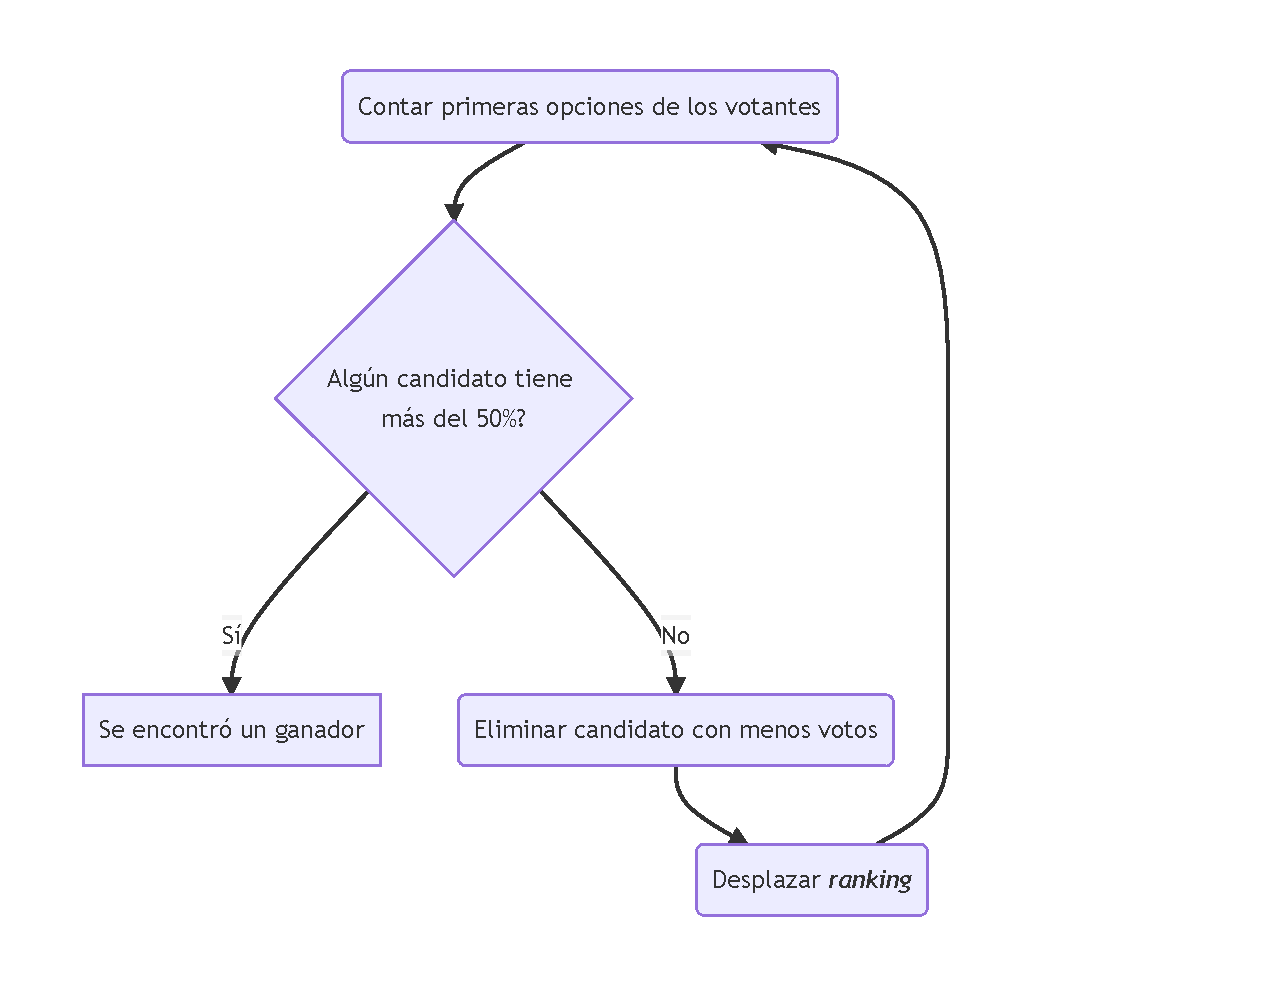
\includegraphics[scale=1.4]{Graphics/irv.pdf}
    \caption{Diagrama de flujo del m\'etodo de desempate instant\'aneo.}
    \label{fig:irv}
\end{figure}

Si m\'as de un candidato posee la menor cantidad de votos, es necesario escoger un m\'etodo de desempate para decidir a cu\'al de ellos eliminar.

\todo[disable,inline]{@TODO esto lleva ejemplo}
\todo[disable,inline]{@TODO decir do'nde se usa esto}

En un sistema de votaci\'on representativa, cada votante emite a lo sumo un voto por un candidato. El voto emitido no se encuentra en forma de lista de preferencias, por ende, no se puede aplicar directamente el m\'etodo de desempate instant\'aneo para determinar un ganador. % No obstante, en  este trabajo se propone una adaptaci\'on de este m\'etodo para sistemas de votaci\'on representativa.

\section{Sistemas Electr\'onicos de Votaci\'on}

Las elecciones tradicionales o basadas en papel son ampliamente
utilizadas alrededor del mundo para la toma de decisiones. Su empleo
destaca en el ámbito político, garantizando durante décadas la
preservación de la democracia en muchos países. Sin embargo, este tipo
de elecciones puede presentar diversos problemas que causan desconfianza
en el electorado \citep{trustworthy_blockchain}. Entre ellos se destacan: 

\begin{enumerate}
\item
  \textbf{fraude pre-electoral:} un ejemplo de ello es cuando
  intencionalmente se manipulan las listas de candidatos para ocultar a
  ciertos partidos. Se han detectado también ilegalidades a la hora de
  confeccionar los distritos de votación, colocando el centro electoral
  en un lugar tan distante que los votantes prefieren no ir a votar. \label{item:fraud}
\item
  \textbf{votos falsos:} en muchos centros electorales no existe una
  verificación biométrica de la identidad del votante, lo cual permite
  con relativa facilidad emitir votos en nombre de personas que no han
  votado.
\item
  \textbf{abuso de poder:} las recompensas y las amenazas son empleadas
  por personas con poder, con el objetivo de coaccionar al votante para
  que elija una opción específica.
\item
  \textbf{conteo de votos sin supervisión:} cuando el conteo no es
  supervisado adecuadamente, es muy probable que no sean contados los
  votos de algunos partidos. \label{item:unsupervised-counting}
\item
  \textbf{falta de auditorías y apelaciones:} las apelaciones y
  solicitudes de auditorías son procesos tan lentos que difícilmente
  suceden antes de las elecciones siguientes. Los candidatos afectados
  suelen entonces llamar a su electorado a protestar y causar
  disturbios, lo cual provoca inestabilidad política.
\end{enumerate}

Todas estas situaciones, y otras que se pueden dar en una elección
convencional, crean descontento y desconfianza entre los votantes.

Un sistema de votación electrónico es capaz de minimizar o solucionar
algunos de los problemas mencionados anteriormente. En un sistema
\emph{online}, por ejemplo, no es necesaria la presencia del votante en
un lugar específico. Luego, la distancia del votante al centro electoral
deja de ser relevante, porque cualquier dispositivo con conexión a
Internet es un ``centro electoral'' y puede estar fácilmente al alcance
del elector. Esto minimiza el problema~\ref{item:fraud}.

En un sistema de votaci\'on electr\'onico se  pueden lograr diversas formas de verificaci\'on biom\'etrica, por ejemplo, mediante la huella digital o el esc\'aner ocular.  Por otro lado, en estos sistemas se puede contar los votos de manera eficiente mientras se van realizando y se  puede publicar en vivo los resultados, lo cual mitiga el problema~\ref{item:unsupervised-counting}.  

Otras bondades poseen los sistemas electrónicos, como son la flexibilidad, lo fácil que pueden ser de usar y lo baratos que resultan con respecto a los sistemas tradicionales. 

Se dice que un sistema electrónico de votaci\'on es centralizado cuando depende de que una agencia central se encargue de registrar, manejar, calcular y revisar los votos. Toda la confianza debe entonces ser depositada en esa agencia, lo cual hace vulnerable al sistema \citep{chica2018weaknesses}. Los sistemas descentralizados constituyen una alternativa en ese sentido. Una de las tecnologías descentralizadas empleadas actualmente es \textit{blockchain}.   Se basa en un registro distribuido e inmutable  de transacciones. Lo que se transacciona puede ser tangible, como lo es  una casa o un carro,  o intangible, como el derecho de autor de una obra o el voto de un elector por un candidato (\cite{blockchain-ibm}). La inmutabilidad y seguridad de este registro se basan en principios de  criptografía, descentralizaci\'on y mecanismos de consenso (\cite{blockch-security-ibm}). 

Existen algunos sistemas de votación electrónicos que emplean \emph{blockchain}, como es Agora \citep{agora}, y muchas propuestas como son \emph{Open Vote Network} \citep{ovn} y la de \cite{borda_count}. Ninguno de ellos soporta un sistema de votaci\'on representativa.

\subsection{Requisitos}

En la presente sección se muestran los requisitos principales que debe cumplir todo sistema de votación electrónico, seg\'un \cite{wang2017review}. Adicionalmente, se presentan otros requisitos opcionales que contribuyen a aumentar la calidad del sistema.

\subsubsection{Principales}

\begin{itemize}
\item
  Correctitud: los votos deben ser contados correctamente. Para ello,
  dos propiedades deben satisfacerse:

  \begin{itemize}
  \item
    totalidad: todos los votos válidos deben ser contados.
  \item
    robustez: los votos no autorizados o inválidos no deben ser
    contados.
  \end{itemize}
\item
  Privacidad: no se conoce la decisión del votante.
\item
  Prevención del doble voto: un votante no puede emitir la misma boleta
  dos veces. También se debe evitar que un tercero pueda clonar una
  boleta previamente emitida por un votante, para registrarla de nuevo a
  nombre de ese votante.
\item
  Elegibilidad: s\'olo los votantes autorizados pueden votar.
\item
  Robustez: poder lidiar con una cierta cantidad de comportamientos
  incorrectos por parte de los votantes o con una falla parcial del
  sistema (un sistema distribuido resiste mejor este tipo de fallas).
\item
  Verificabilidad individual: el votante debe poder verificar que su
  voto haya sido contado.
\item
  Usabilidad: se le debe facilitar a los usuarios del sistema la
  utilización de este a lo largo del proceso de votación, auditoría y
  consulta. El usuario debe poder lograr su cometido con la menor
  cantidad de recursos y la mayor satisfacción posibles.
\end{itemize}

Se desea que el sistema de votaci\'on representativa a implementar cumpla con los requisitos: correctitud, prevenci\'on del doble voto, eligibilidad, robustez y verificabilidad individual.

\subsubsection{Adicionales}

\begin{itemize}
\item
  Justeza: no se calculan los resultados hasta el fin de la votación.
\item
  Incoercibilidad: evitar la coerción (e.g.~votación en cadena o
  \emph{chain voting} (Jones 2005)).
\item
  Eficiencia: el sistema debe responder con rapidez ante una gran
  cantidad de votantes y elecciones.
\item
  Movilidad: se puede votar desde dispositivos móviles.
\item
  \emph{Vote-and-Go:} que se pueda votar \emph{offline} una vez la
  boleta haya sido emitida.
\item
  Verificabilidad universal: cualquier persona puede verificar que los
  votos hayan sido contados correctamente.
\item
  Verificabilidad de extremo a extremo (\emph{end-to-end} o E2E): al
  votante se le entrega un recibo que demuestra que votó, pero no indica
  cuál fue su decisión.
\end{itemize}

Se desea que el sistema de votaci\'on representativa a implementar cumpla con los requisitos: eficiencia y verificabilidad universal.